\documentclass[prc,twocolumn]{revtex4}
\usepackage{epstopdf}
\usepackage{amsmath}
\usepackage{graphicx}

%\usepackage{dcolumn}
%\newcolumntype{d}[1]{D{.}{.}{#1} }
%\newcolumntype{t}[1]{D{-}{-}{#1} }

\hyphenpenalty=1500
\exhyphenpenalty=1500

\begin{document}

\title{Characterizing and analyzing Hammamatsu multianode photo multiplier tubes for use in the RICH detector in the Jefferson Lab Hall B CLAS12 spectrometer}

\author{~Cameron Clarke$^1$}
\author{Jenna Samuel$^2$}
\author{Valery Kubarovsky$^3$}
\author{Andrey Kim$^3$}
\affiliation{$^1$Mississippi State, $^2$Florida International University,\\ $^3$Thomas Jefferson National Accelerator Facility}

\begin{abstract}
	
	The Large Acceptance Spectrometer (CLAS12) at the Thomas Jefferson National Accelerator Facility will use a ring-imaging Cherenkov (RICH) detector. RICH is designed to measure the velocity of near-light speed particles from nuclear and particle interactions by detecting the tens of photons emitted as Cherenkov radiation. It is imperative that enough of the Cherenkov photons be detected by photomultiplier tubes (PMTs). The detector requires a high spatial resolution for identifying rings and measuring their radii, used to facilitate particle identification. PMT producer Hamamatsu continues to develop new, smaller, high-gain, multianode PMTs (MAPMTs) which may be able to achieve the necessary sensitivity, resolution and gain desirable in the CLAS12 RICH detector. Hamamatsu develops several of these new MAPMTs, including their H8500 and newer H12700 models, and we sought to determine which was best suited for use in the RICH detector. First we studied the MAPMTs' single photoelectron (SPE) spectra, dark current, and crosstalk to determine which MAPMT design was better. We built a test bench and automatic system for data acquisition, analysis and database storage and we also implemented two fitting procedures for this data. This will be used for characterization of all PMTs in the CLAS12 RICH detector. We show that the Hamamatsu H12700 PMTs are more suitable for use in the CLAS12 RICH detector in regards to resolution of the single photoelectron spectrum, average number of photoelectrons, and dark current and we also showed the necessity of a new fit to model the behavior of PMTs which are near the pedestal and with few photons. We saw that although there is little difference in dark current, the H12700 PMTs suffer less from crosstalk, have narrower SPE spectra, and have efficiencies. We see that the relative efficiency is average 29(5) percent higher in H12700 than H8500 MAPMTs. We find that the new fit better describes the data for H12700 PMTs, providing a more accurate, and a seemingly more physically meaningful model of the MAPMTs performance. These results mean that the H12700 MAPMTs will increase the efficiency of the RICH detector. Although there are some concerns about below average pixels on the edges of the tubes, we find that the H12700s should prove useful across the field of Cherenkov ring measurements and particle identification.
	
\end{abstract}

\date{\today}

\maketitle

\section{Introduction}

	\subsection{Physics}
	
		\begin{figure}
			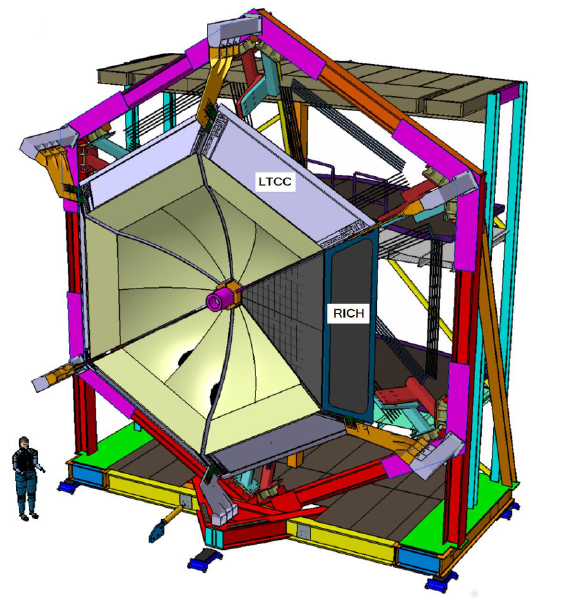
\includegraphics[width=1.0\linewidth]{RICHclas12.png}
			\caption{ne sector of the RICH detector in the CLAS12 Spectrometer. \cite{CDR}}
			\label{CLAS12}
		\end{figure}
		
		As part of the ongoing study of the structure of nucleons in Hall B at the Thomas Jefferson National Accelerator Facility (JLab), the Large Acceptance Spectrometer (CLAS12), shown in Figure \ref{CLAS12}, aims to accurately identify the secondary particles of high energy reactions, assist in probing the strangeness frontier, and aid in characterizing transverse momentum distribution (TMD) and generalized parton distribution (GPD) functions. \cite{CDR}  Indispensable to this task is the ability to identify kaons, pions, and protons.  With the CLAS12 spectrometer providing accurate momentum measurements the RICH detector provides tandem Cherenkov lightcone radius measurements which yield the velocities of near light-speed particles, thus facilitating mass-dependent particle identification.
		
		\begin{figure}
			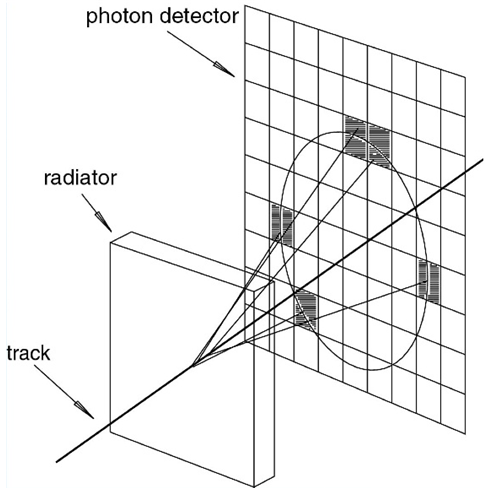
\includegraphics[width=0.9\linewidth]{cherenkov.png}
			\caption{Simplified schematic of a RICH. \cite{CDR}}
			\label{cherenkov}
		\end{figure}
		
		\indent The RICH detector takes advantage of Cherenkov radiation which is the phenomenon of light emission by particles traveling through a medium faster than the speed of light in that medium, such that
		$$v \geq \frac{c}{n}$$
		where $n$ is the refractive index of the medium, and  $\beta=\frac{v}{c}$ is the velocity of the particle as a fraction of $c$, the speed of light in vacuum. Cherenkov photons are produced as the passing particle excites an electromagnetic shockwave in the medium. Photons are produced in a cone with opening angle $\theta_{c}$ as shown in Figure \ref{cherenkov} and described by
		\begin{equation}
			cos(\theta_{c}) = \frac{1}{\beta n(\lambda)}
			\label{theta}
		\end{equation}
		where $n(\lambda)$ is the index of refraction dependent on the emitted photons' wavelength. The number of Cherenkov photons emitted per unit $L$ of the medium for wavelength $\lambda$ is given by
		\begin{equation}
			\frac{d^{2} N}{d L d \lambda} = \left( \frac{2 \pi \alpha Z^{2}}{\lambda^2}\right) sin^{2}(\theta_c)
			\label{section}
		\end{equation}
		where $\alpha$ is the fine structure constant and $Z$ is the electric charge of the particles. 
		\\
		\indent Precise velocity measurements can be obtained from the Cherenkov angle which, when paired with the momentum information from the CLAS12 tracking system allows for confident particle identification. To get a confident lightcone radius measurement for determining the opening angle the RICH detector must be composed of elements with a high efficiency for detecting single photons, with little noise, and with a high spatial resolution.  These needs are magnified by the rather small number of Cherenkov photons that are actually produced per event.
		
	 \subsection{Multi Anode Photomultiplier Tubes}
	 
		\indent The RICH detector will utilize around 400 multi-anode photomultiplier tubes (MAPMTs) with 25000 channels in total, aerogel as a Cherenkov radiator, and mirrors for additional light focusing. \cite{CDR}  Hamamatsu designs MAPMTs which use the dynode structure shown in Figure \ref{MAPMT} to provide the necessary spatial resolution greater than that available from traditional PMTs while maintaining a high sensitivity to single photons and low noise or dark current.  MAPMTs are better for our stated purpose than traditional photomultiplier tubes (PMTs) because they have a much higher spatial resolution as a result of their internal design and the multiple anode channels, or pixels, on the same device.  These MAPMTs are also better than silicon photomultipliers (SiPMs) that are very good at detecting single photons, in regard to dark current noise among other factors.
		\\
		\indent Initially, the Hamamatsu H8500 MAPMT model was chosen as the best option because they provide high quantum efficiency for visible light and sufficient spatial resolution (6x6 mm$^2$) at a limited cost.  However, recently Hamamatsu has released the new H12700 MAPMT model which shows enhanced single photoelectron (SPE) detection and is otherwise similar to the H8500 MAPMTs in spatial resolution, cost, and the rest.  Consequently we desire to better characterize the new H12700 MAPMTs and choose the best model between these two options for inclusion in the CLAS12 RICH.
	
		\begin{figure}
			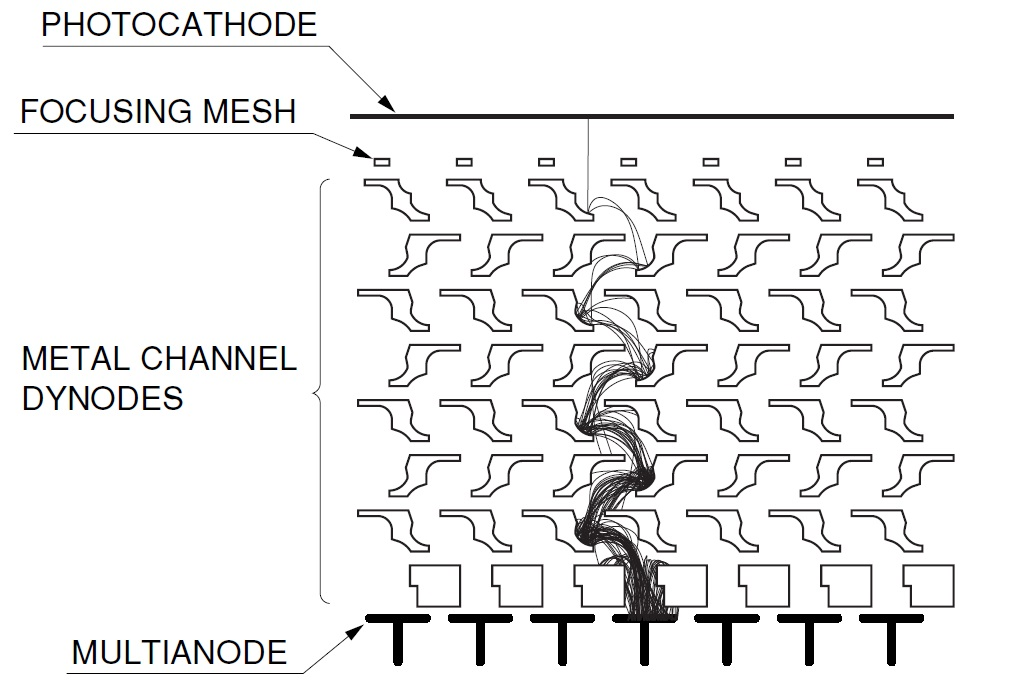
\includegraphics[width=1.0\linewidth]{dynodestructure.jpg}
			\caption{Dynode Structure of MAPMTs showing path of electrons in signal amplification. \cite{hamamatsu}}
			\label{MAPMT}
		\end{figure}


\section{Procedure and Methods}

	\subsection{Experimental Apparatus}
	
		\begin{figure*}
			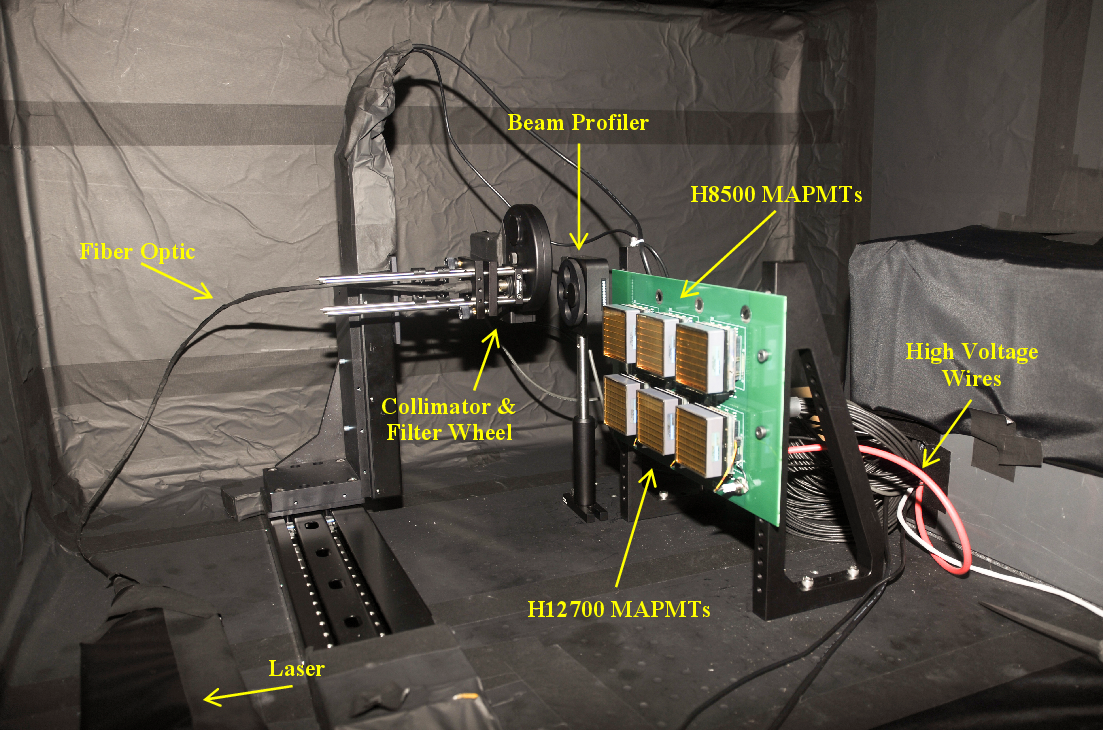
\includegraphics[width=1.0\linewidth]{blackbox.png}
			\caption{Inside of the blackbox and PMT testing bench.}
			\label{blackbox}
		\end{figure*}
		To test MAPMTs and provide characterizations of their response functions we built a blackbox and laser apparatus as shown in Figure \ref{blackbox}. We can connect up to six MAPMTs to circuit board spots, but for the current flash analog to digital converter (fADC) data acquisition (DAQ) setup we look at just two at a time. The laser, filter wheel, high voltage control, and data acquisition are all handled automatically by Bash scripts, and ROOT and C++ executables as shown in Figure \ref{schematic}.	
		\begin{figure}
			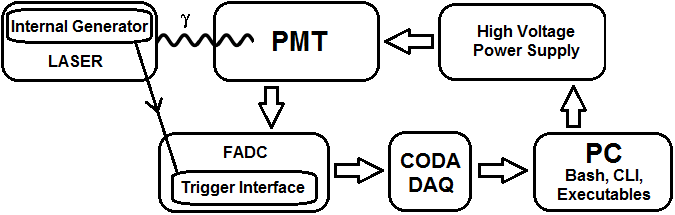
\includegraphics[width=1.0\linewidth]{schematic.png}
			\caption{Schematic diagram of data acquisition system.}
			\label{schematic}
		\end{figure}
		\\
		\indent We operated a 470 nm laser and trigger at 10 kHz frequency with a fiber collimator attached to the neutral density filter system to decrease the number of multiple photon events.  For each of the 64 pixels of the MAPMTs 100,000 events were collected for 4 high voltage settings within Hamamatsu's suggested range (-1000, -1050, -1075, and -1100 volts).  We used the standard CEBAF Online Data Acquisition system (CODA) for collecting our data. Each event is stored in ROOT tree files which are later analyzed with ROOT. For MAPMT comparison purposes we looked at 80 H8500 model and 10 of the H12700 model and investigated crosstalk, anode dark current, the average number of photoelectrons ($\mu$), the average value of the SPE signal (Q$_1$), and the relative efficiency, which is the number of events 5$\sigma$ above the Gaussian pedestal. 

	\subsection{A new mathematical model}

		\begin{figure*}
			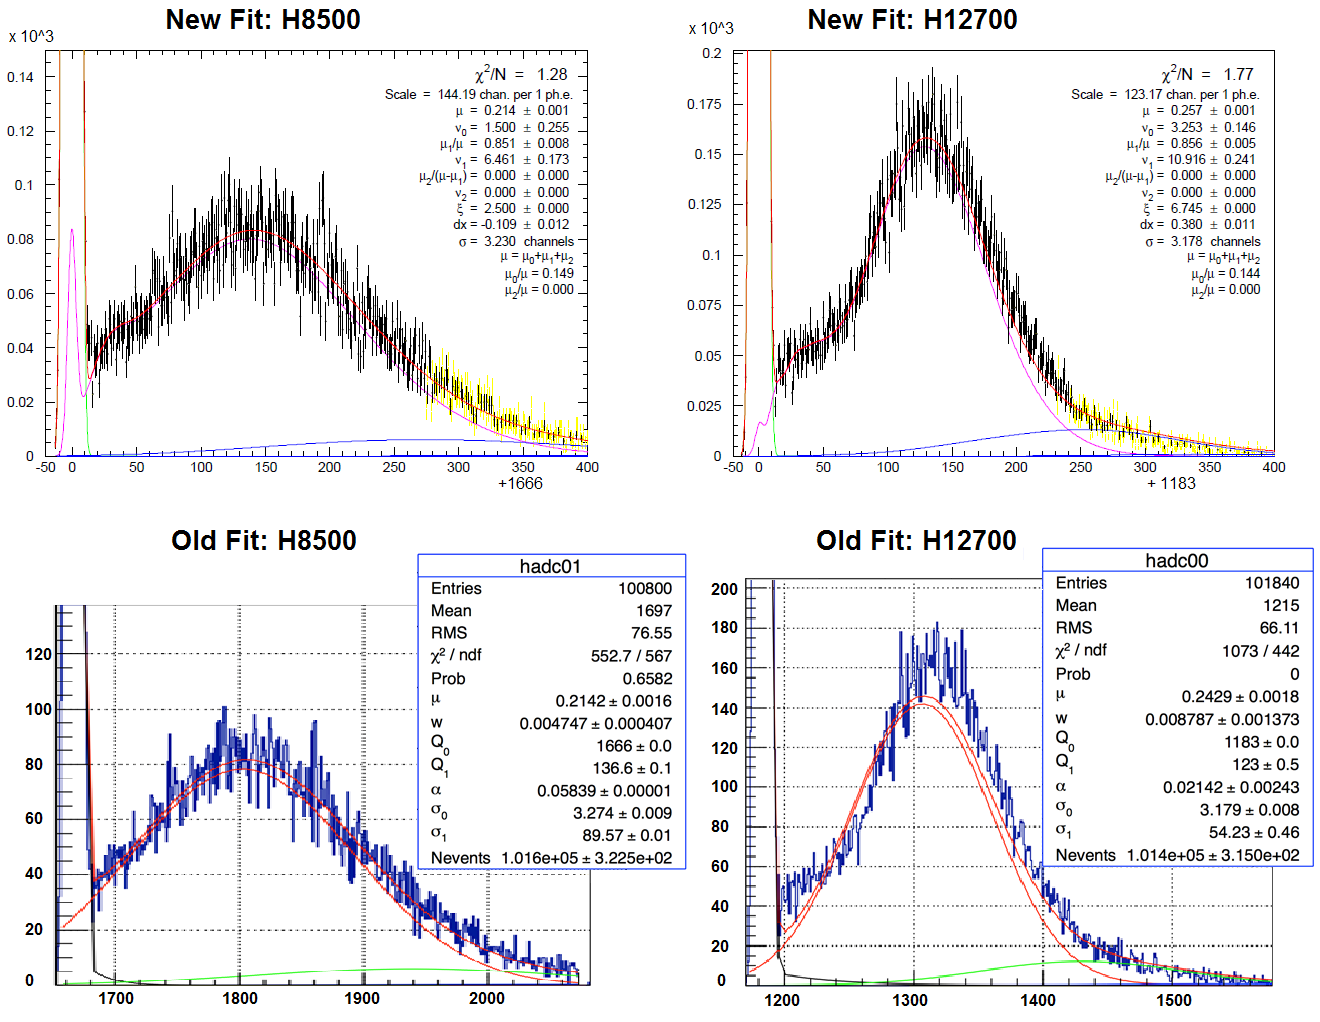
\includegraphics[width=1.0\linewidth]{comparison2.png}
			\caption{Comparison of Poissonian and Gaussian fits for H8500 	and H12700 MAPMTs.} 
			\label{comparison}
		\end{figure*}
		We started by using a model for signal amplitude distribution based off of Gaussian single photoelectron spectra as discussed in Bellamy et al. (1994)\cite{bellamy} that works reasonably well for H8500, but this model does not satisfactorily treat the spectra seen in the new H12700 MAPMTs from Hamamatsu. Consequently, Pavel Degtyarenko at JLab has developed a more complicated model using several Poisson components to better fit the MAPMT spectra, especially in the single photoelectron cases. \cite{pavel}  
		\\ 
		\indent The general expression for Pavel's model of the PMT response or signal amplitude distribution is given in Equation \ref{model} and represents a parameterized function of a trinomial average of discrete two-stage compound Poisson distributions convoluted with an ideal first stage measurement Gaussian distribution ($\mathrm{G}(\mathrm{A},n)$), 
		\begin{equation}
		\label{model}
		p \mathrm{(A)}= \sum\limits_{n=0}^{\infty} \left \{
		\mathrm{G}(\mathrm{A},n)
		\sum\limits_{m=0}^{\infty} \left [ \mathrm{P}(\mu;m)
		\mathrm{T}_{\mathrm{av}}(m,n) \right ] \right \}
		\end{equation}
		where $p$(A) is the probability distribution of the measured spectra normalized s.t. 
		$$\int\limits_{-\infty}^{\infty} \mathrm{P(A)}d\mathrm{A}=1,$$
		with $$\mathrm{A} = (\mathrm{A}_{measured} - \mathrm{A}_{pedestal})/scale,$$
		wherin $A_{measured}$ and $A_{pedestal}$ are the amplitudes of the measured signal and pedestal values in flash Analog to Digital Converter (fADC) units and $scale$ is a factor in ADC units such that the average amplitude of single photoelectron signals is equal to one: $\mathrm{A}_{1 ph.e.} = 1 $.  The parameter $\mu$ is the average number of photoelectrons obtained from  $m$ Poissonian fit components $$\mathrm{P}(\mu;m) = \frac{\mu^{m} e^{-\mu}}{m!}$$ whose value can ultimately be used to find the scale by 
		$$ scale = \frac{ \langle \mathrm{A}_{\mathrm{meas}} - \mathrm{A}_{\mathrm{ped}} \rangle}{\mu}. $$
		\indent The components from $n$ unique numbers of electrons coming off the first dynode as a function of $m$ incident electrons onto the first dynode also are described by $n$ Poissonians
		$$\mathrm{P}(m \nu;n) = \frac{(m \nu)^{n}\  e^{-m \nu }}{n!}$$
		which can be used to replace the $\mathrm{T}_{\mathrm{av}}(m,n)$ term in Equation \ref{model}.  This new model is comprised of multiple compound Poisson distributions for the different numbers of incident and outgoing electrons from the first dynode as well as a Gaussian pedestal.  The software utilizes the MINUIT numerical minimization computer program written in Fortran and outputs plots of the MAPMTs and their parameters with PAW.  Additional specification on the mathematics of this new model can be found in Degtyarenko, P. (2014). \cite{pavel}
		\\
		\indent Pavel's fitting code was implemented using the database Jenna Samuel built and was applied to all the available data and the resultant fit parameters were stored in the database.  Examples of the two fits for both Hamamatsu H8500 and H12700 MAPMT cases are shown in Figure \ref{comparison}.  This new model provides a functional form that ideally more accurately describes the spectra and which, to the eye, is a better fit particularly in the H12700 case as seen on the right side of Figure \ref{comparison}.  Such a model which is more realistic and physically meaningful is important for the newer H12700 MAPMTs' as their spectra are less accurately approximated by Gaussians, potentially leading to futility when trying to quantify a measure of their width vs. gain or some other measure of single photoelectron detection efficiency.  Additionally, since the RICH detector will be using nearly 400 MAPMTs it matters that a good model capable of describing the single photoelectron spectrum be available for further characterization of so many detector components. 
	
	\subsection{Software}
		
		The automated data collection and analysis software originally written by Andrey Kim was modified and expanded for further functionality in comparing MAPMT varieties and for characterizing individual MAPMTs. We wrote Bash scripts which execute user customizable data collecting runs without requiring intimate familiarity with the code.  We constructed a database using Bash scripts and wrote analysis software for storing lists of data files corresponding to particular data runs and measurement types and for storing the resultant fit parameters.  ROOT analysis executables were produced that take data from the runtable and rundata database and produce plots of the fit parameters for visual inspection. All of these are interconnected and rely on each other or the user for input as shown in Figure \ref{software}.
		
		\begin{figure}
			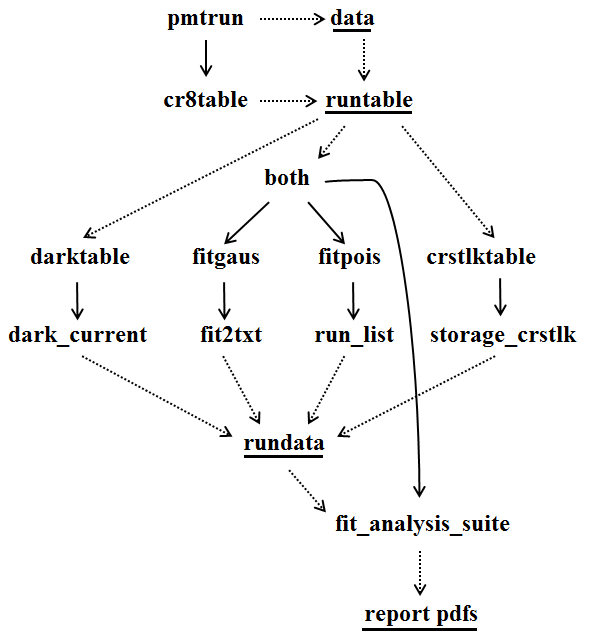
\includegraphics[width=0.8\linewidth]{software.png}
			\caption{A simplified software hierarchy and modularity scheme. Solid lines represent one function calling another and dashed lines represent reading or writing files. Underlined is data storage and everything else is a bash script or ROOT executable.}
			\label{software}
		\end{figure}
		
		\indent Most of these programs may be edited to promote further functionality and ease of use, but following is a simple summary of the programs and their input and output.

		\subsubsection*{Data Collection Bash Scripts}  		
		\indent Principally the $pmtrun$ script allows the user to manipulate, using command line flags, the data run characteristics of dark sleep time, the pmt serial number(s) and name(s), the number of events to take, whether or not to use the laser, which pixels to look at including the option to leave the laser stationary at the home position, and the voltage(s) to utilize.  Further documentation for this and the other bash scripts is available by either using the flag -h for help or for ROOT executables by executing the program with no command line input at all. 
		\\
		\indent The main program $pmtrun$ also calls the $darkrun$ script which is a simplified version of $pmtrun$ that explicitly runs a dark current measurement by leaving the laser off, collecting a million events, and optionally using an initial dark sleep time. Both $pmtrun$ and $darkrun$ use a program called $hv$, with simple offshoots $hvon$ and $hvoff$, which is another bash script that controls the high voltage computer and lets the user change any of the PMTs' voltages within acceptable ranges. Additionally these data acquisition programs communicate with the $pcal0$ computer and store the data in the \underline{data} folder in the $rich$ computer.  For database storage $pmtrun$ calls another program called $cr8table$ that intelligently creates \underline{runtable} database entries based off of special or default user input. 
		
		\subsubsection*{Fitting and Data Extraction}	
	\begin{figure}
		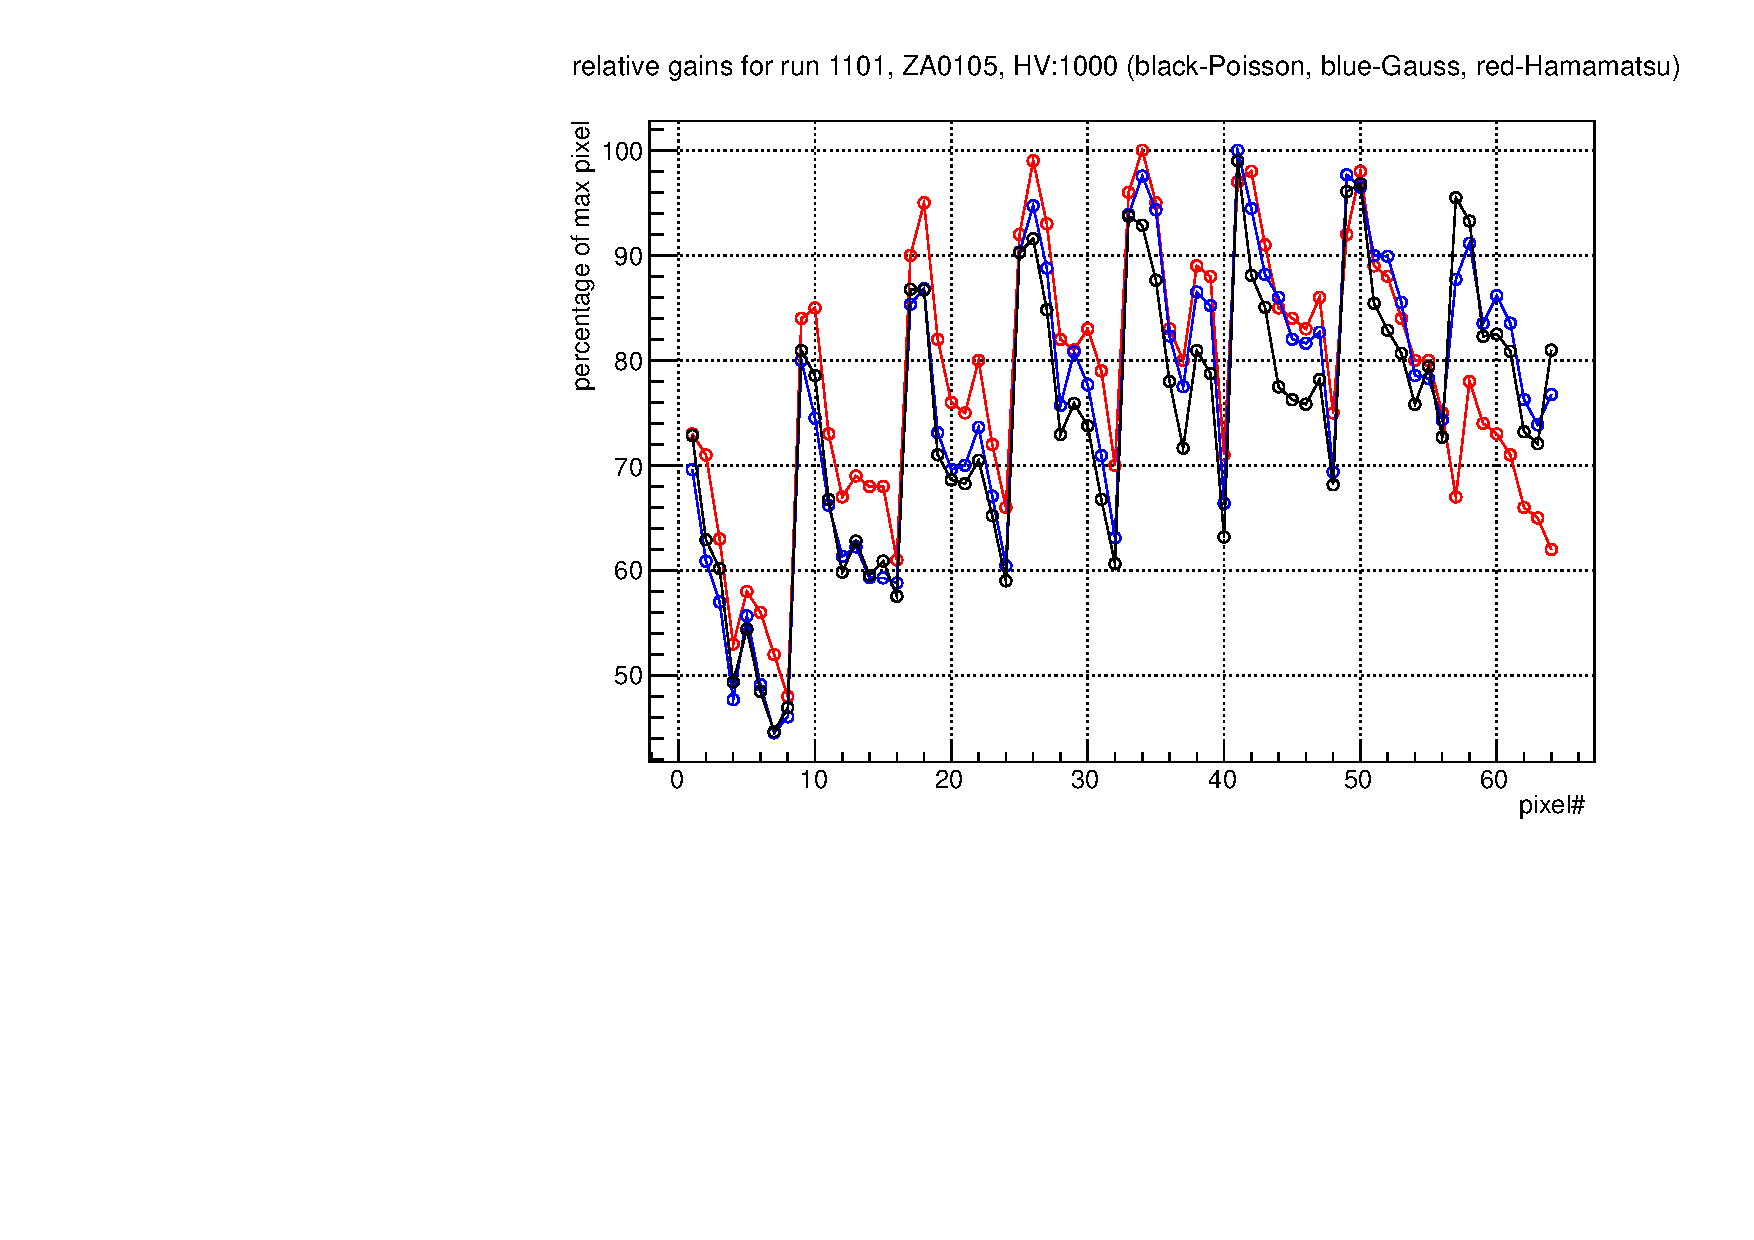
\includegraphics[width=1.0\linewidth,page=1]{newreport_1101.pdf}
		\caption{Relative gains for a Hamamatsu H12700 MAPMT at 1000 volts. The Poissonian model's gain is obtained from the fit parameters s.t. gain $= scale \cdot \mu$.}
		\label{hamamatsu}
	\end{figure}
	\begin{figure}
		\includegraphics[width=1.0\linewidth,page=2]{hamamatsu.pdf}
		\caption{Gain as a function of high voltage for a H12700 MAPMT.}
		\label{gainhv}
	\end{figure}
	\begin{figure}
		\includegraphics[width=1.0\linewidth,page=3]{hamamatsu.pdf}
		\caption{$\chi^{2}_{\nu}$ as a function of high voltage for a H12700 MAPMT.}
		\label{chi2hv}
	\end{figure}
	\begin{figure}
		\includegraphics[width=1.0\linewidth,page=4]{hamamatsu.pdf}
		\caption{$\mu$ as a function of high voltage for a H12700 MAPMT.}
		\label{muhv}
	\end{figure}
	\begin{figure}
		\includegraphics[width=1.0\linewidth,page=7]{hamamatsu.pdf}
		\caption{Gain ratios at different voltages for a H12700 MAPMT.}
		\label{hv}
	\end{figure}

		\indent Fitting the data collected and stored in \underline{data}  utilizes the \underline{runtable} database which contains a list of the ROOT data files and their intended data types.  The bash script $both$ reads all acceptable ``Gain'' runtable entries and runs the old Gaussian and new Poissonian fits, stores the resultant fit parameters and other information in a folder called \underline{rundata}, and makes a PDF from the Poissonian fit's data for visual inspection. The script $both$ runs $fitgaus$ which is another bash script that takes one \underline{runtable} entry at a time and executes the ROOT executable $fit2txt$ which adds a line for each ROOT tree \underline{data} file examined into a \underline{rundata} text file named after the \underline{runtable} entry number. The script $both$ also calls the bash script $fitpois$ which is similar to $fitgaus$ in making text \underline{rundata} entries but must be run as the fit@rich user and uses the PAW and Fortran program $run\_list$ to fit the same PMT with Pavel's new Poissonian fit.  
		\\
		\indent The data file that $fit2txt$ generates is similar in size, data type, and ordering to the file generated automatically by Pavel's fit in its $run_list$; $fit2txt$ appends one new line each time it is run for a \underline{runtable} entry pixel where the line is an array containing the following information as floating point numbers in the following order: blank, blank, PMT serial number, blank, voltage, pixel number, gain, $\chi^{2}_{\nu}$, $\sigma_{pedestal}$, $\mu$, number of photoelectrons, $\sigma_{gain}$, the total number of events observed, $\alpha$, $\omega$, pedestal position, the mean value of all the events, efficiency, blank, blank, blank, blank, blank, blank, blank, blank, blank, blank.
		\\
		\indent The bash scripts $darktable$ and $crstlktable$ are similar to $fitgaus$ as they take a \underline{runtable} entry and execute the ROOT executables $dark\_table$ and $storage\_crstlk$ respectively on the ROOT tree \underline{data} files to generate \underline{rundata} entries with arrays that contain dark current and crosstalk information for their \underline{runtable} entry inputs.
		\\
		\indent Of the several PDF generating programs, the one which should be used for analyzing PMTs and determining their quality is the $fit\_analysis\_suite$ ROOT executable which takes a \underline{runtable} input and reads the necessary \underline{rundata} storage text files and generates a PDF that shows the measured gain (from the Poissonian fit) vs. the Hamamatsu data sheet gains as well as several of the fit parameters for each pixel at the different high voltages, described in detail below.  There are several other programs that can be used to generate PDFs for visual analysis, including the program $new\_analysis\_suite$ which is similar to $fit\_analysis\_suite$ except that it displays side by side the old Gaussian fit and the new Poissonian fit values. The program $mu\_difference$ plots the Poissonian fit's $\mu$ values for two different \underline{runtable} entries on the same graph.  Similarly $efficiency\_difference$ calculates the relative efficiency, a measure of the number of events over pedestal when a pixel is illuminated vs. the total number of events, for two different \underline{runtable} entries for comparison.  The program $fit\_efficiency\_difference$ is hard coded to make similar graphical comparisons of the fit derived single photoelectron efficiencies for four specific MAPMTs' data that have similar high and low gains and should be modified heavily with new SPE spectrum information from Pavel's fit to perform this task automatically or for other MAPMTs.  
		\\
		\indent These are all of the important new ROOT and Bash programs produced for automated data collection, storage and analysis in their current state and further information can be found by reading their help documentation and the source codes themselves (found in the $/home/rich/richdev/$ folders).  Example output of the first page of the results from $new\_analysis\_suite$ is shown in Figure \ref{hamamatsu} and examples of gains for different voltages, $\chi^{2}_{\nu}$, $\mu$, and gain ratios are also shown in Figures \ref{gainhv} through \ref{hv}, showing these programs' and PDFs' utility for visually checking the quality of MAPMTs.

	\subsubsection*{Example Software Usage}
		
		For example, to collect, store, fit, and produce PDFs for normal gain and dark current measurements of two PMTs in the blackbox at once, the user would do the following:
		\begin{itemize}
			\item Execute $pmtrun$ on the command line by entering ``pmtrun CA7686 ZA0175''
				\subitem Among other automatic things this takes normal measurements with the default $pmtrun$ settings and also executes $darkrun$ for both PMTs.
				\subitem Additionally this will automatically call the $cr8table$ script that stores the resultant ROOT \underline{data} files' names in a new \underline{runtable} entry.
			\item As the fit@rich user execute $fitpois$ to perform the new Poissonian fit and store the results into the \underline{rundata} database by entering at the command line ``fitpois 1225'' or whatever the \underline{runtable} interesting number is. 
			\subitem To generate a report PDF then enter to the command line ``fit\_analysis\_suite 1225''
			\item Or the user can simply execute the program $both$ with the \underline{runtable} entry's run number which does both steps in the above point and also generates the Gaussian fit's text file. This would be entered on the command line as ``both 1225''
			\subitem This also generates the corresponding report PDF file for the Poisson fit parameters.
		\end{itemize}
		Additionally the user could write a script (or use the scripts called $run\_all$ or $check\_all$ found in the \underline{rundata} directory) which looks at every single valid \underline{runtable} entry and runs the $both$ script for them. Let the user take caution however, as the text files that the $fitgaus$ and $fitpois$ scripts ultimately handle are not rewritten upon future executions but are simply appended to, meaning that successive executions of this code will just add more, superfluous data to the files.  Conditional logic steps may be taken to eliminate this hazard by checking in the $both$ script, before proceeding, if the particular text files exist already, but this has not yet been attempted.
		
\section{Results}

	\begin{figure*}
		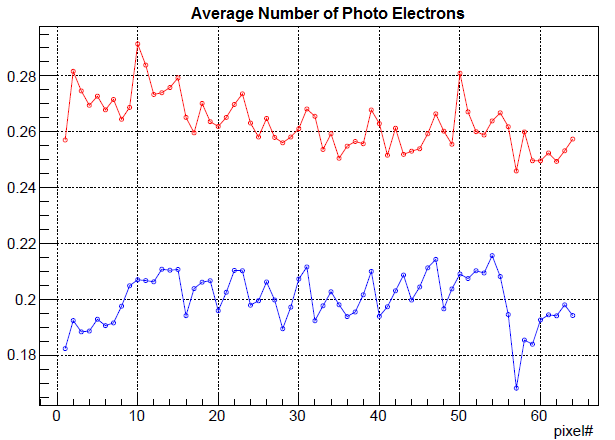
\includegraphics[width=0.45\linewidth]{highmu.png} \hspace{0.1in} 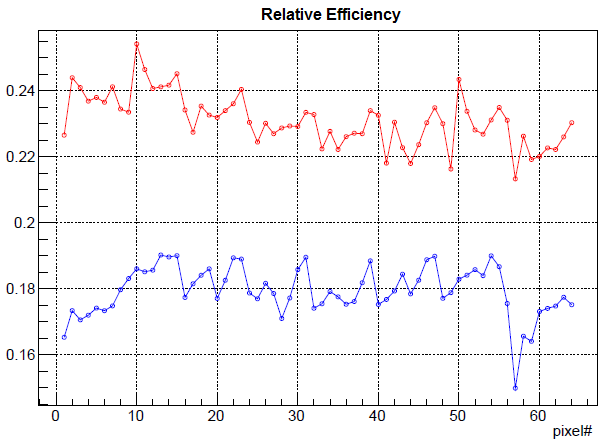
\includegraphics[width=0.45\linewidth]{highefficiency.png}
		\\
		\vspace{0.1in}
		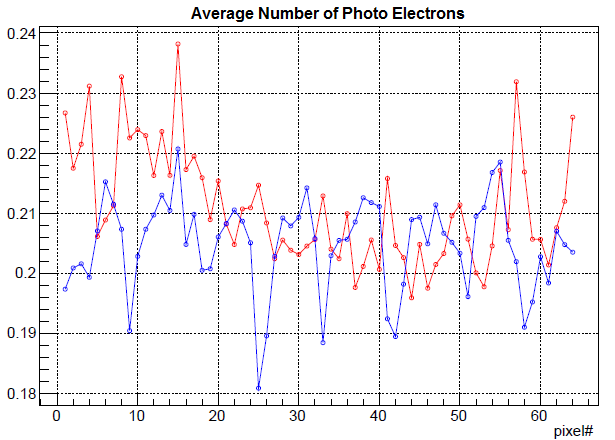
\includegraphics[width=0.45\linewidth]{lowmu.png} \hspace{0.in}
		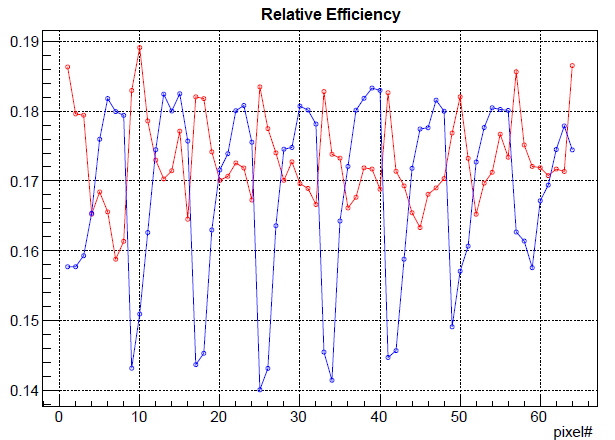
\includegraphics[width=0.45\linewidth]{lowefficiency.png}
		\caption{$\mu$ (average number of photoelectrons) and relative efficiency in arbitrary units, at 1075 volts, for two similar high gain MAPMTs above, and two similar low gain MAPMTs below. Red is model H12700, Blue is H8500.}
		\label{efficiency}
	\end{figure*}

	We tested 80 H8500 and 10 H12700 Hamamatsu MAPMTs and obtained spectral and dark current data for all 64 pixels at 4 different high voltages for each. Looking at the $\chi^{2}_{\nu}$ of both fit techniques using the data of all 10 of new H12700 and 80 old H8500 MAPMTs, all 64 pixels for each, and all 4 high voltages, we see that Pavel's new Poissonian model is better for the H12700 MAPMTs in terms of $\chi^{2}_{\nu}$ on average by $15$ percent, as $\chi^{2}_{\nu} = 2.7$ on average for the new fit instead of $3.2$ for the old fit. Additionally, in the case of H8500 MAPMTs, the new fit is about as good as the old Gaussian model. A comparison of the normalized gains for the two fits compared to the Hamamatsu data is given in Figure \ref{hamamatsu} and shows that the in regards to the MAPMTs' pixels' responses and gain the new fit is at least as good as, if not better than, the old Gaussian fit.
	\\	
	\indent  We saw that although there is little difference in crosstalk signals, the H12700 PMTs suffer less from dark current, have narrower SPE spectra, and have higher $\mu$ and relative efficiency values. An example plot of the $\mu$'s and relative efficiencies of H8500 and H12700 PMTs with similar low and high gains is shown in Figure \ref{efficiency}.
	\\	% Mention the fit efficiency?
	\indent We see that the relative efficiency is closely related to the $\mu$ which is on average, over all pixels at all voltages for all the PMTs we tested, $29\pm5$ percent higher in H12700 than H8500 MAPMTs. One concern with these $\mu$ measurements however is that the laser system used to measure these PMTs was only incident on a portion of each pixel, consequently missing their sum total effect and pinpointing possible spatial dependencies which should be further studied and perhaps remeasured with a fully illuminated MAPMT instead of collimated pinpoint laser light. In terms of crosstalk for the two varieties of MAPMT the H12700s appear to be better than the H8500s. The H12700s have a decrease in crosstalk by nearly a factor of two. Additional studies of dark current in the H12700s would be useful, as the dark current is usually dominated by individual pixels or bad regions of the PMT instead of spread around evenly like in the H8500s, but overall the two varieties are not very different in terms of dark current.

\section{Conclusion}
	We find that Pavel's fit better describes the data for H12700 PMTs, providing a more accurate, and a seemingly more physically meaningful model of the MAPMTs performance. Our findings of similar crosstalk, dark current and gain for both MAPMTs while we see the average $\mu$ a good deal larger with similarly increased relative efficiencies for the H12700 MAPMTs suggests that they are better suited for use in the CLAS12 detector than the H8500 MAPMTs. Consequently, this higher overall performance ability of H12700 MAPMTs for all RICH detectors should continue to be investigated to answer questions of SPE efficiencies and spectrum inhomogeneities.
	\\
	\indent The tighter SPE spectral shape and higher average $\mu$ mean that the H12700 MAPMTs should increase the efficiency of the RICH detector in detecting single Cherenkov photons. Although there are some concerns about below average pixels on the edges of these tubes and fine structure to the pixels themselves that merit further study, we find that the H12700s should prove useful across the field of Cherenkov ring measurements and particle identification.
	
	
\section*{Acknowledgements}
	
	I would like to thank the U.S. Department of Energy, SULI, JLab, and the RICH and CLAS12 collaborations as well as their member institutions. I would also like to thank Dr. Dipankgar Dutta and Dr. Jim Dunne for encouraging me to come to JLab. I would also like to thank my family and friends for facilitating my travels throughout the summer research experience.
	
\begin{thebibliography}{99}

	\bibitem{CDR} \textit{The RICH Conceptual Design Report}, (2013)
	\bibitem{hamamatsu} \textit{PMT Handbook}, Hamamatsu \textbf{3a}, 169 (2007)
	\bibitem{bellamy} Bellamy, E.H., et. al., \textit{Absolute calibration and monitoring of a spectrometric channel using a photomultiplier}, Nuc. Inst. \& Meth. in Phys. Res. A \textbf{339}, 468-476 (1994)
	\bibitem{pavel} Degtyarenko, P., \textit{Parameterization of Amplitude Response Functions Measured by Photon Detectors}, JLab Tech Note Repositorium (2014)	
	
\end{thebibliography}

\end{document}